\section{パルス印加実験の結果と考察}

\subsection{電流パルスを用いたα相からβ相への変換}
図\ref{fig:181228_before_after_pulse_log}に電流パルス印加前後の抵抗値を示す。パルス印加前(赤色)の抵抗は温度を小さくしながら測定したもので、温度が小さくなるほど抵抗が小さく、半導体的な温度-抵抗依存性を示す。

一方、パルス印加後の抵抗(青色)は60Kより低温で温度が小さくなっていることがわかる。この領域で金属からの寄与が大きく、超伝導体転移が確認できた。

では金属との並列として理解できる\cite{Mayr,McLachlan}

\begin{figure}[!h]
 \begin{minipage}{\hsize}
    \begin{center}
   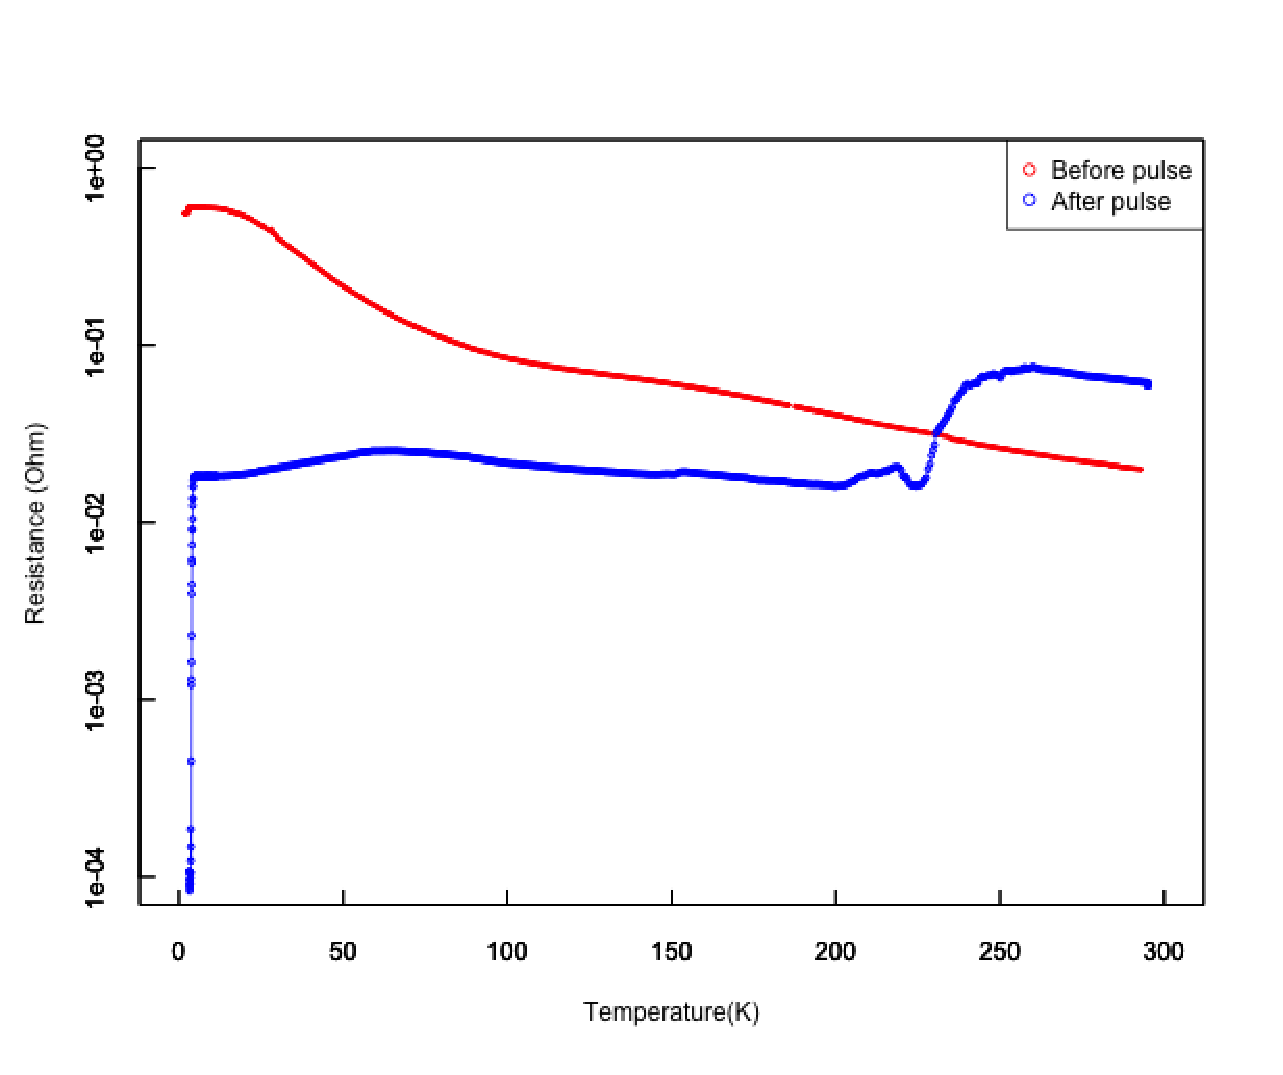
\includegraphics[width=\hsize]{results_discussions/181228_before_after_pulse_log.eps}
  \end{center}
  \caption{}
  \label{fig:181228_before_after_pulse_log}
   \end{minipage}
 \begin{minipage}{0.5\hsize}
    \begin{center}
   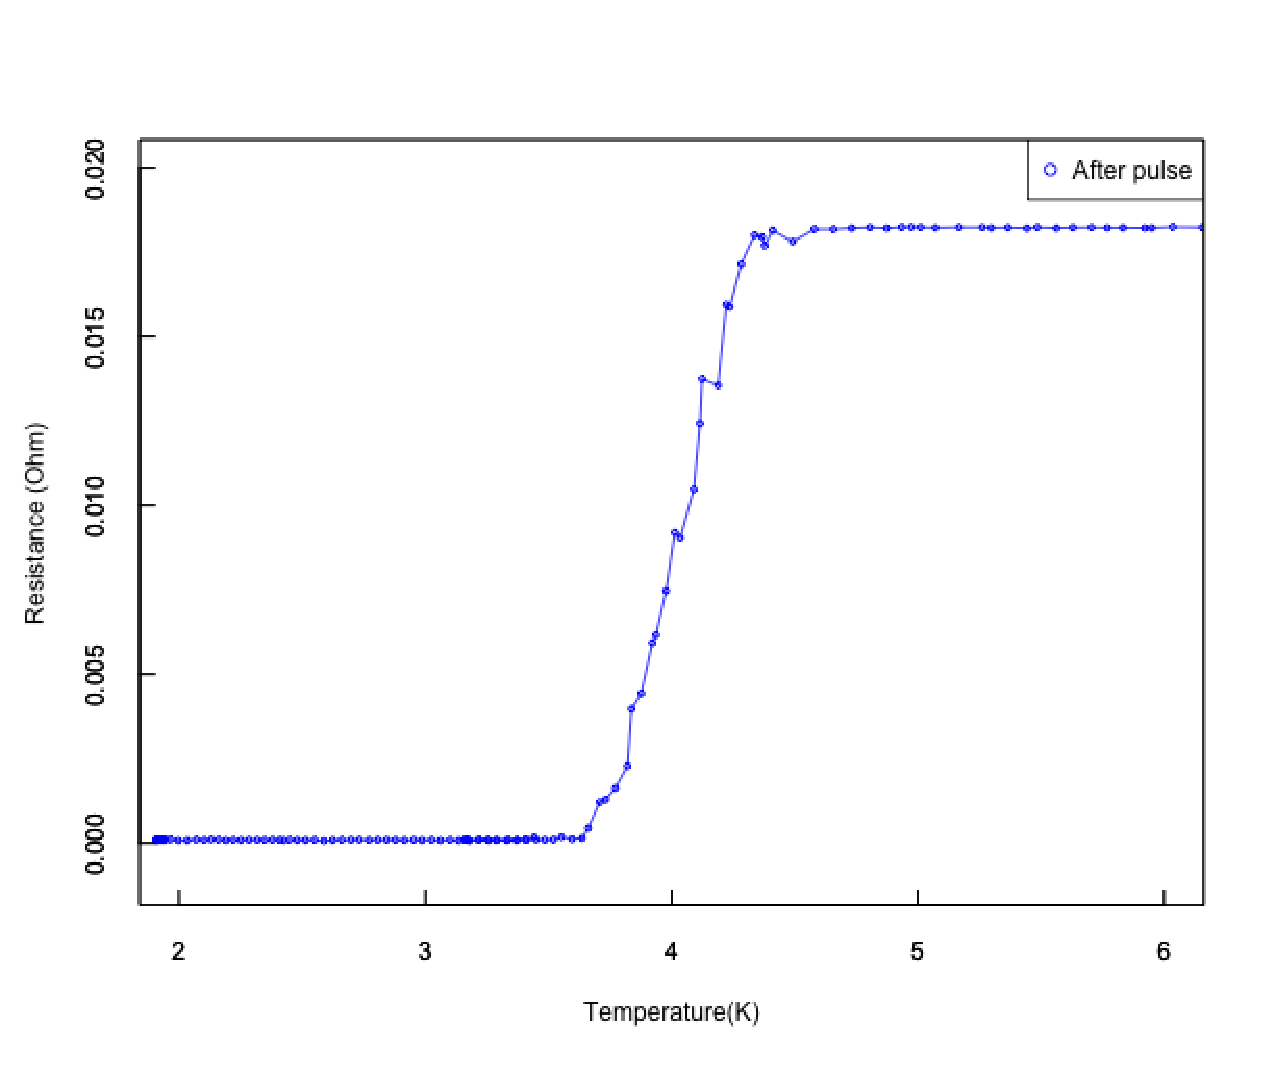
\includegraphics[width=\hsize]{results_discussions/181228_after_pulse.eps}
  \end{center}
  \caption{}
  \label{fig:181228_after_pulse}
 \end{minipage}
 \begin{minipage}{0.5\hsize}
     \begin{center}
   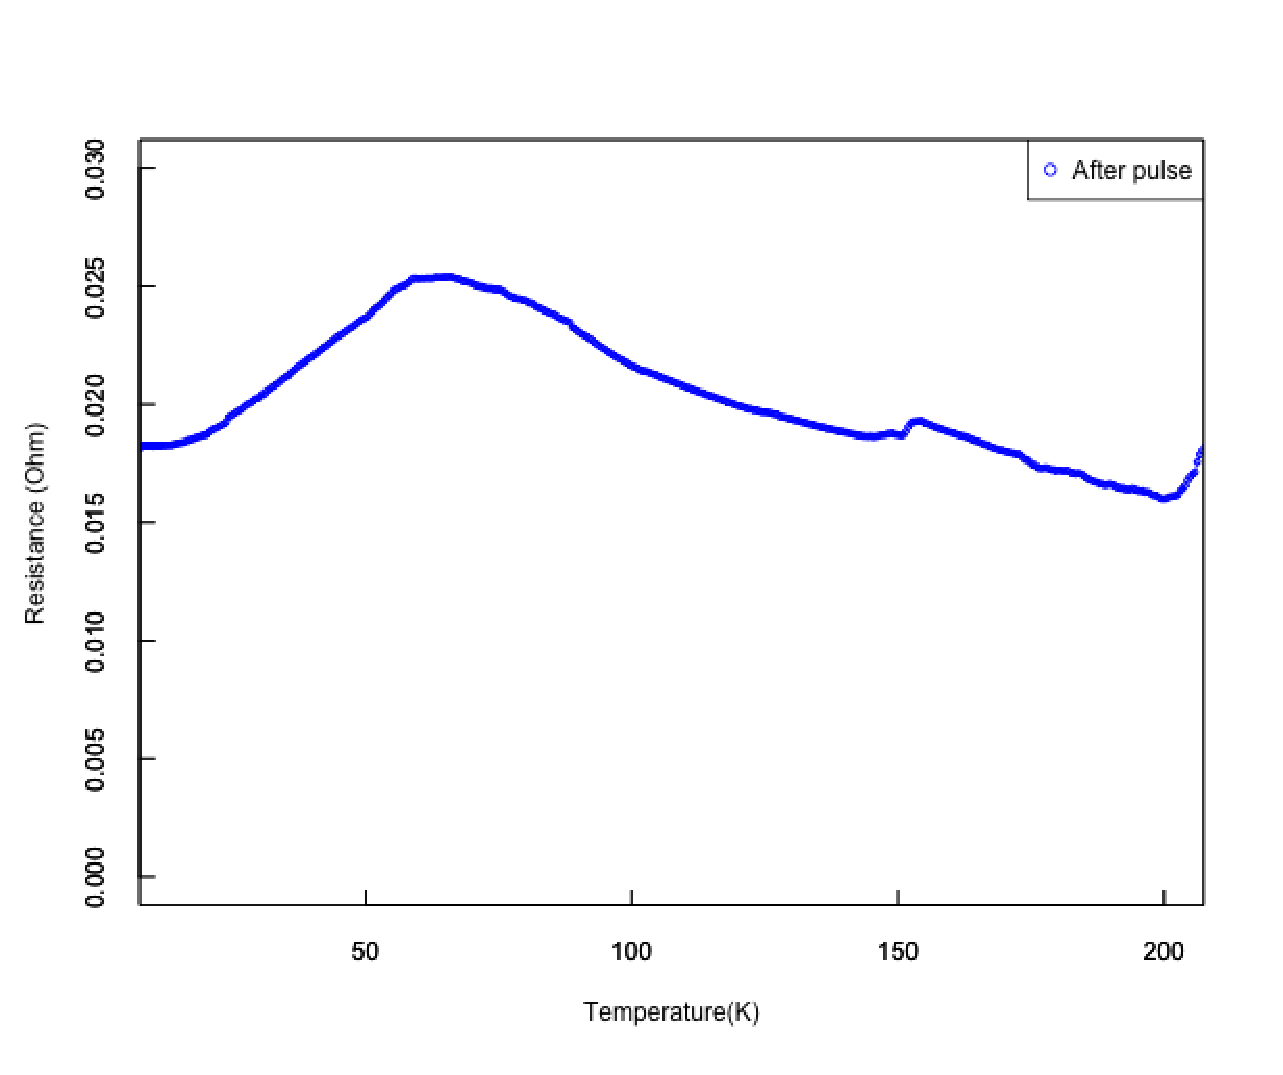
\includegraphics[width=\hsize]{results_discussions/181228_after_pulse2.eps}
  \end{center}
  \caption{}
  \label{fig:181228_after_pulse2}
   \end{minipage}
\end{figure}


\begin{figure}[!h]
 \begin{minipage}{\hsize}
    \begin{center}
   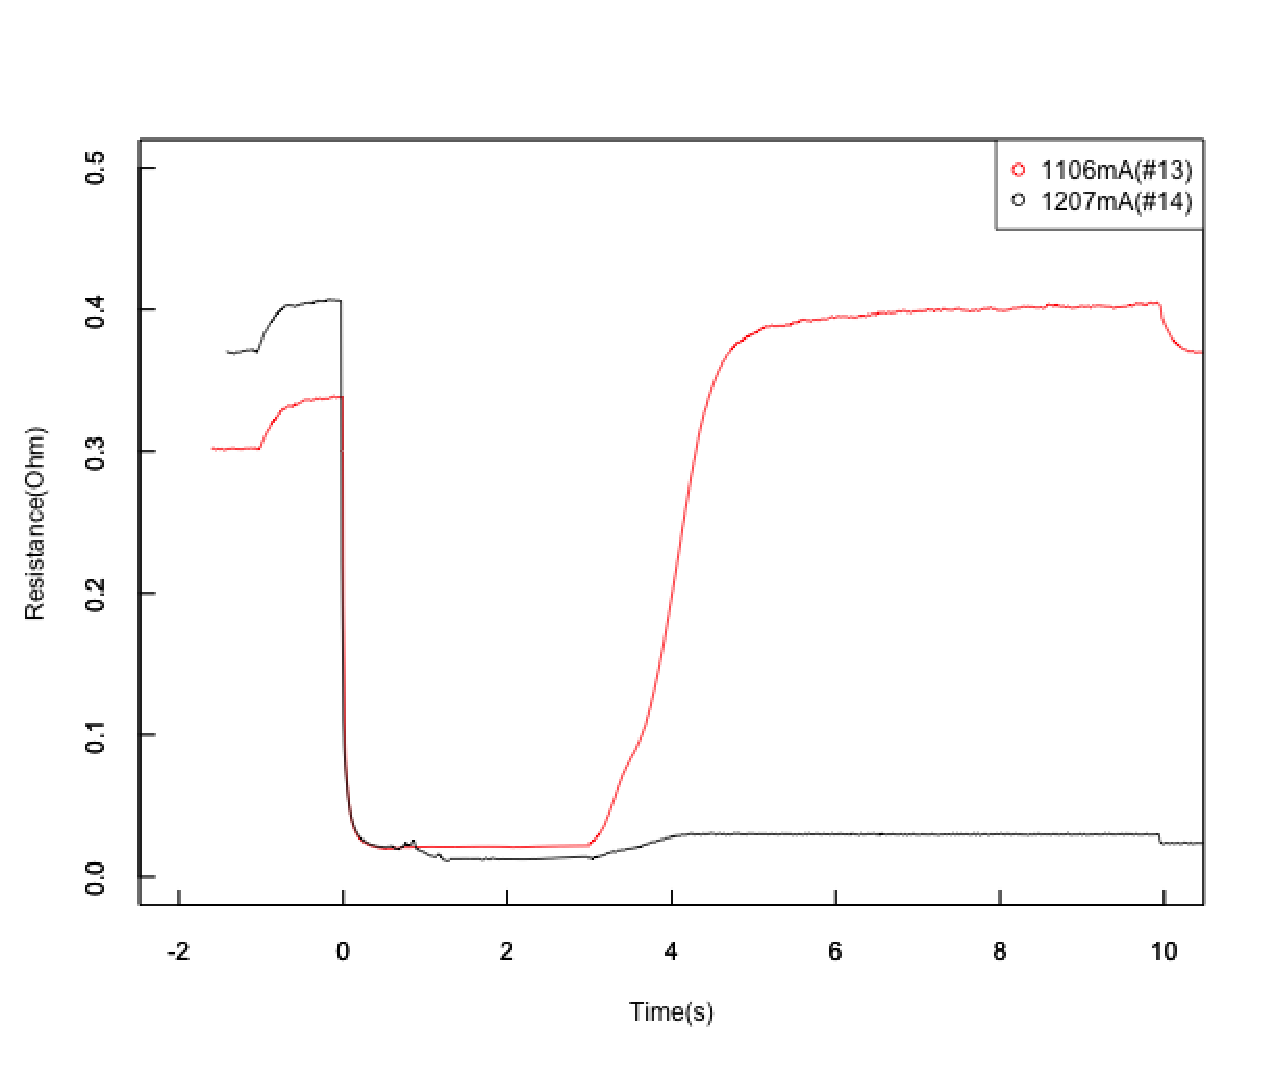
\includegraphics[width=0.7\hsize]{results_discussions/181228_Resistance_pulse_selected.eps}
  \end{center}
  \caption{}
  \label{fig:181228_Resistance_pulse_selected}
 \end{minipage}
 \begin{minipage}{\hsize}
     \begin{center}
   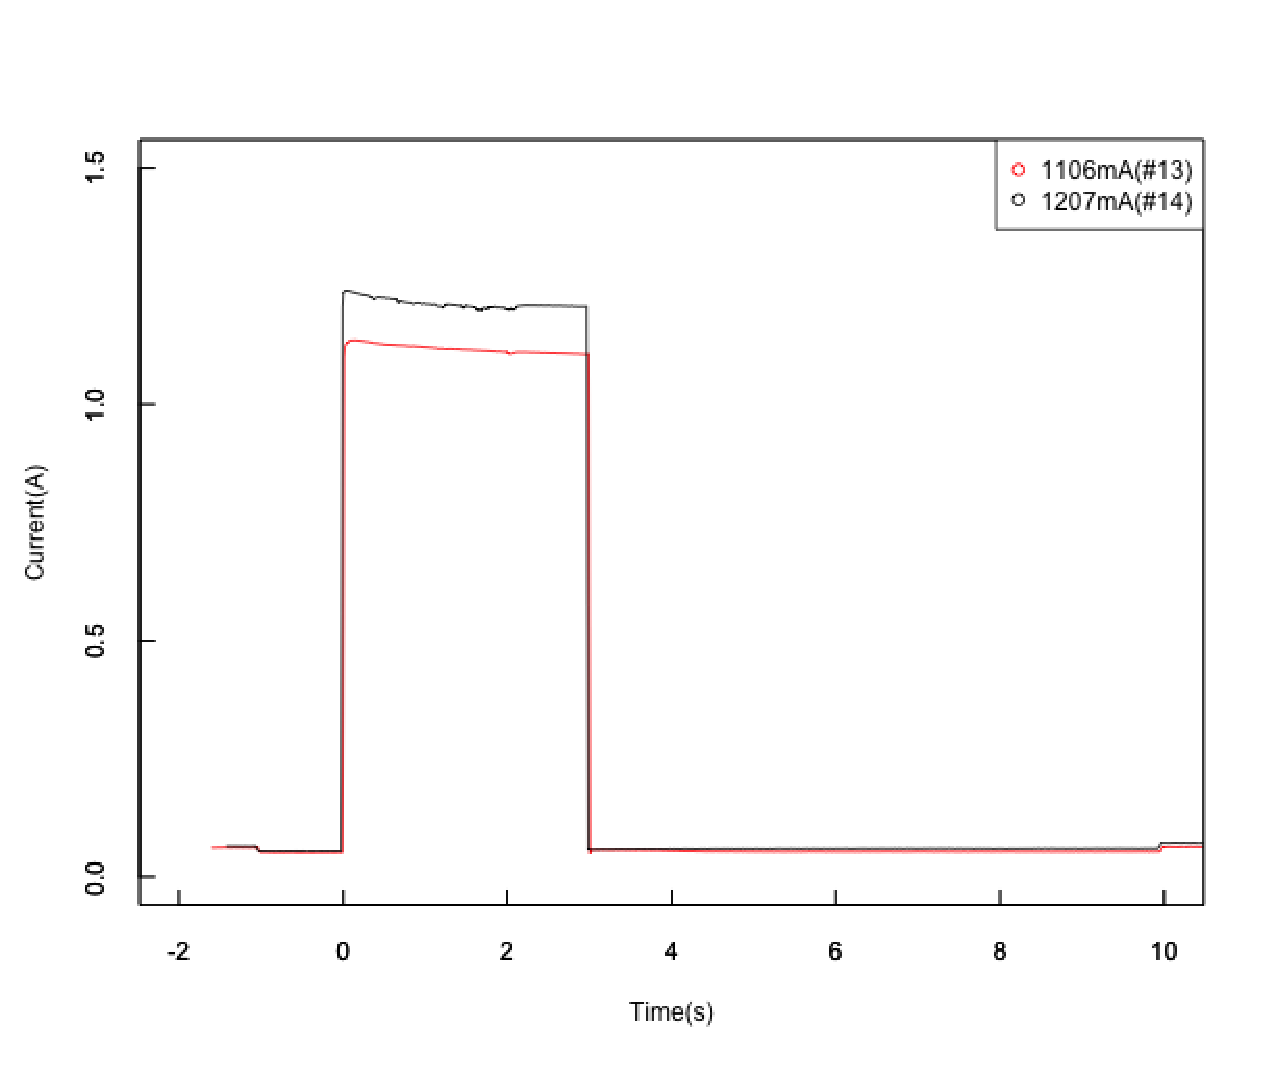
\includegraphics[width=0.7\hsize]{results_discussions/181228_current_pulse_selected.eps}
  \end{center}
  \caption{}
  \label{fig:181228_current_pulse_selected}
   \end{minipage}
\end{figure}

\subsection{電流パルスによるα相とβ相の共存状態の生成}
\begin{figure}[!h]
 \begin{minipage}{\hsize}
    \begin{center}
   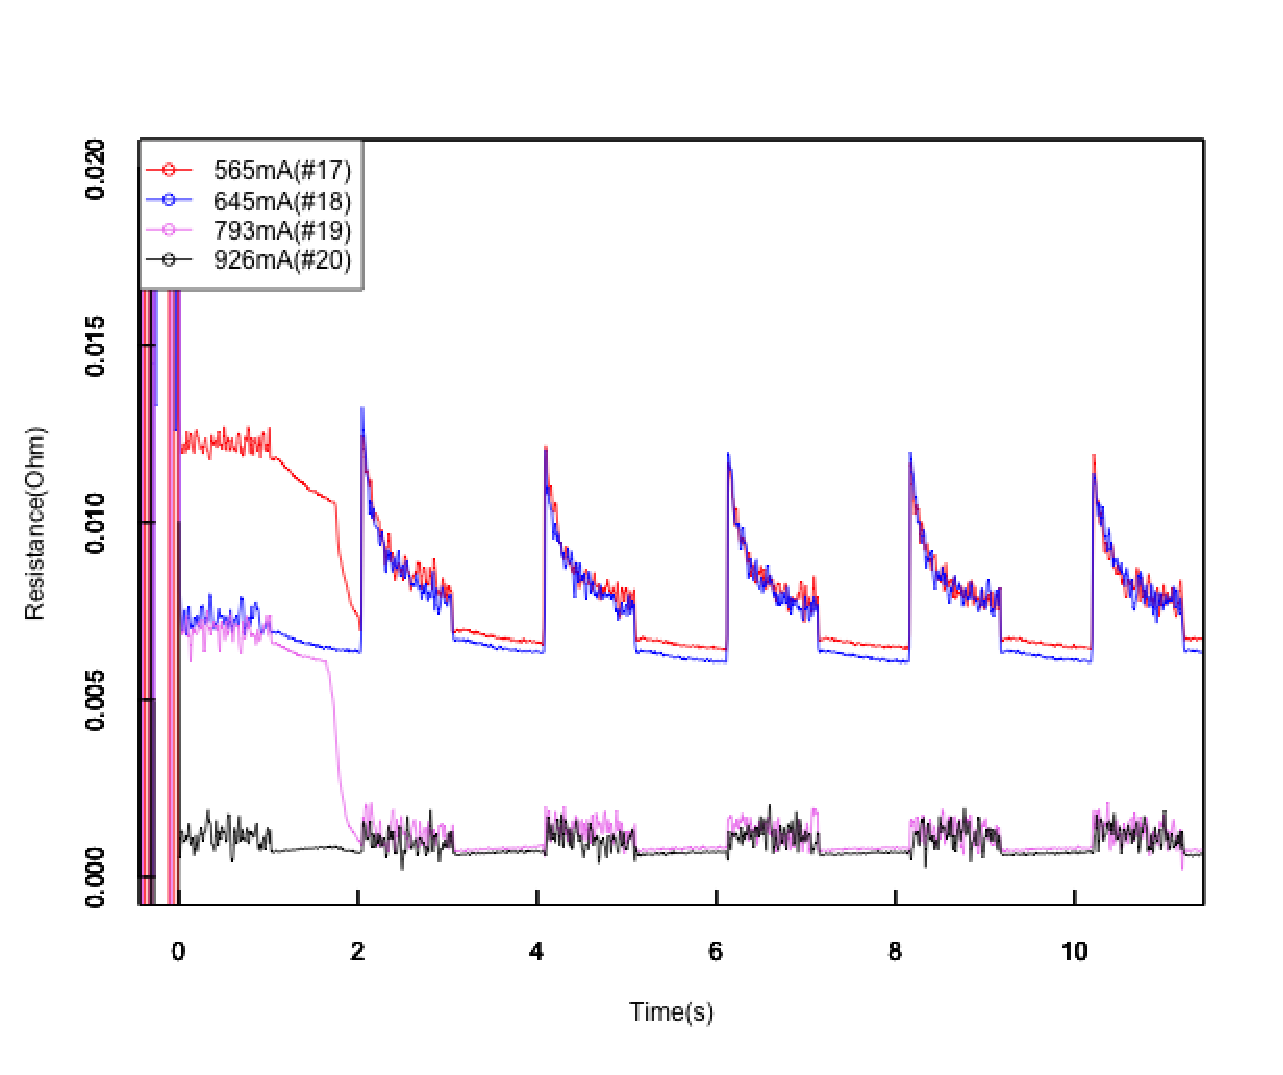
\includegraphics[width=0.9\hsize]{results_discussions/190112_Resistance_pulse.eps}
  \end{center}
  \caption{}
  \label{fig:190112_Resistance_pulse}
 \end{minipage}
 \begin{minipage}{\hsize}
     \begin{center}
   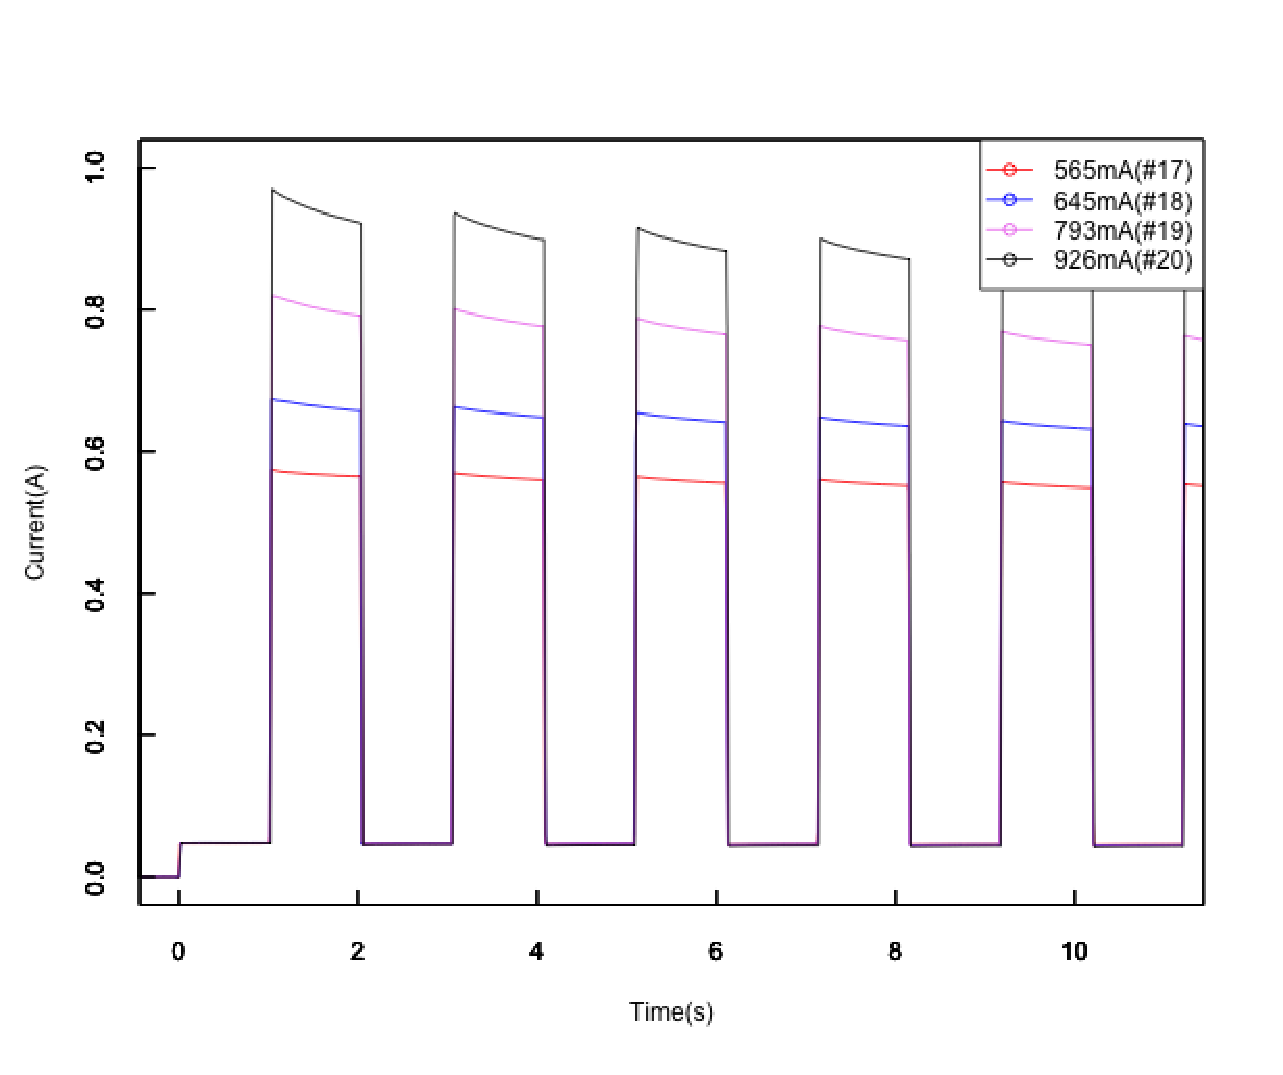
\includegraphics[width=0.9\hsize]{results_discussions/190112_Current_pulse.eps}
  \end{center}
  \caption{}
  \label{fig:190112_Current_pulse}
   \end{minipage}
\end{figure}

パルス印加中とパルス印加前後の試料の顕微鏡写真を図\ref{fig:190112_before_pulse17}から図\ref{fig:190112_after_pulse20}に示す。写真は顕微鏡で撮影した動画から切り取ってきたものである。動画撮影中のセットアップは変化させなかったが、撮影後、相転移が見やすくなるように露出とコントラス、色調を調整した。
\begin{figure}[htbp]
 \begin{minipage}{0.5\hsize}
  \begin{center}
   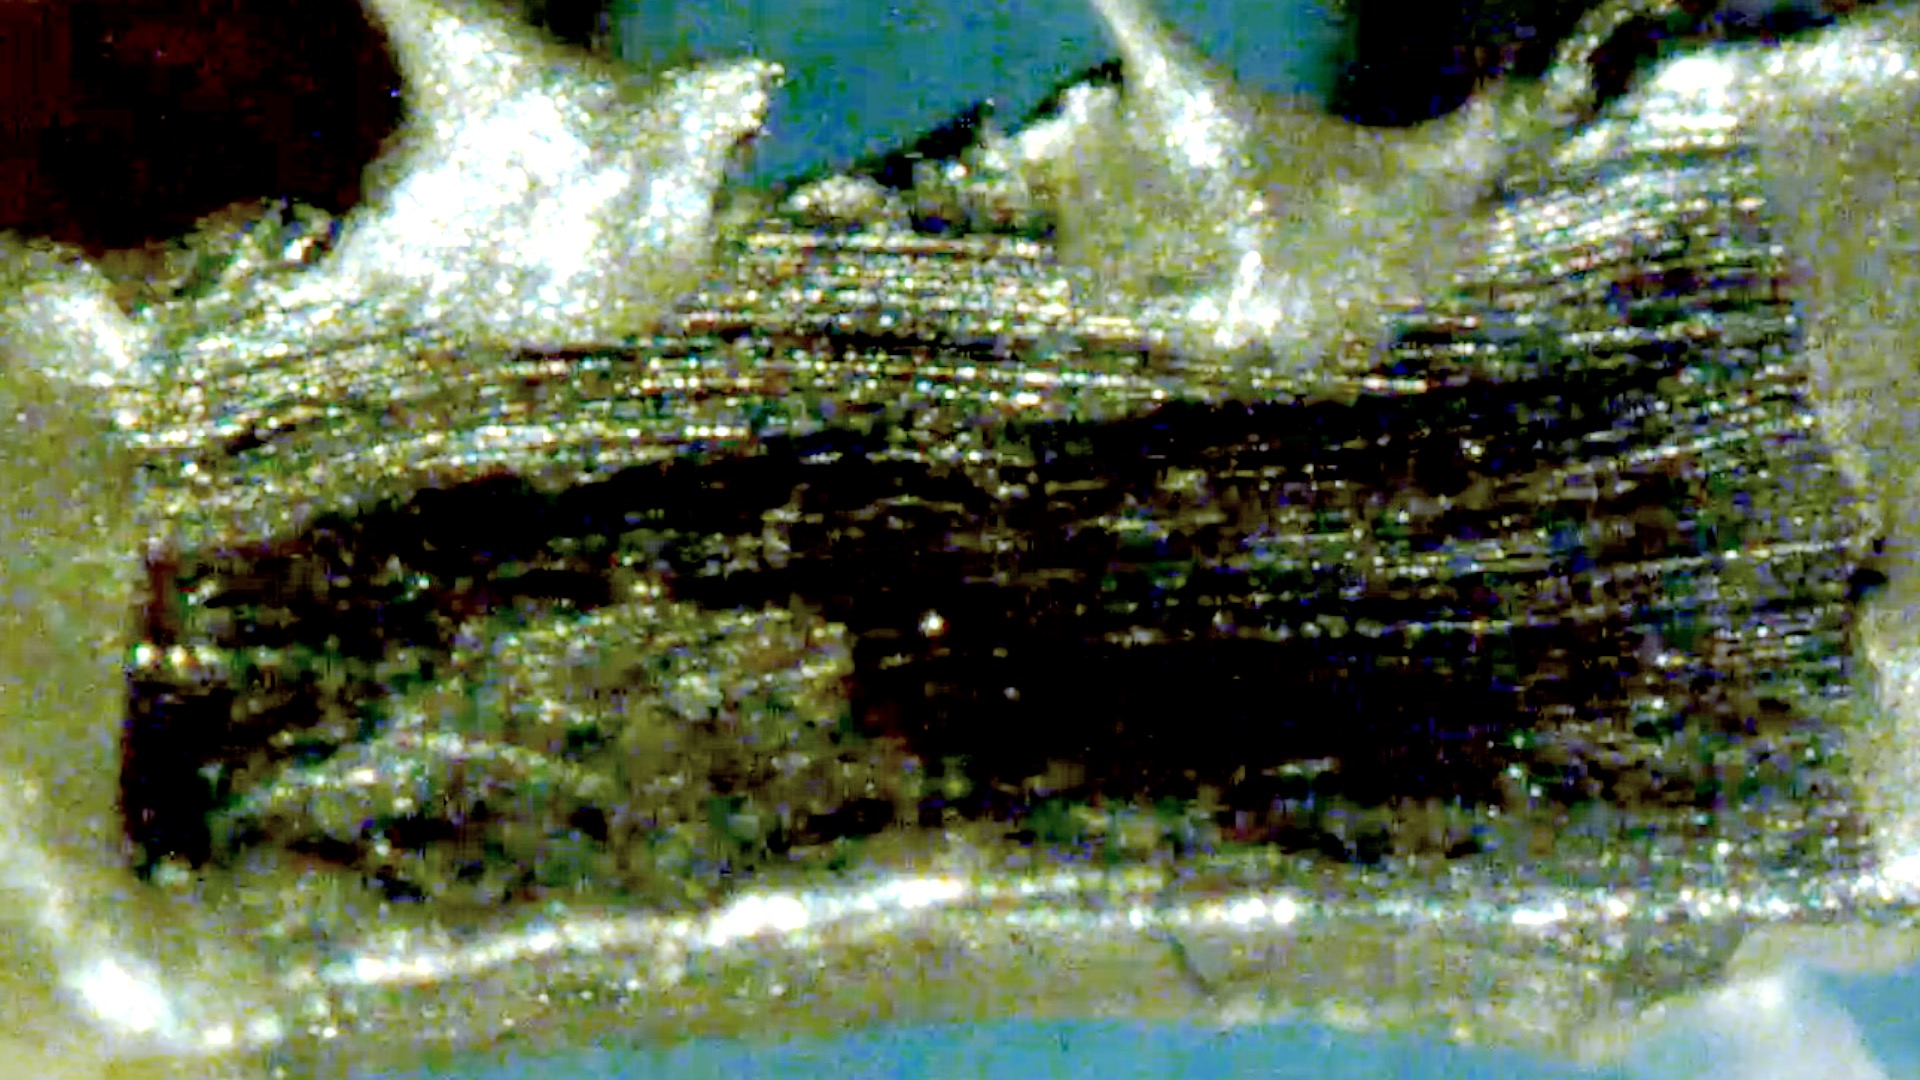
\includegraphics[width=\hsize]{results_discussions/190112_before_pulse17.eps}
  \end{center}
  \caption{}
  \label{fig:190112_before_pulse17}
 \end{minipage}
 \begin{minipage}{0.5\hsize}
  \begin{center}
   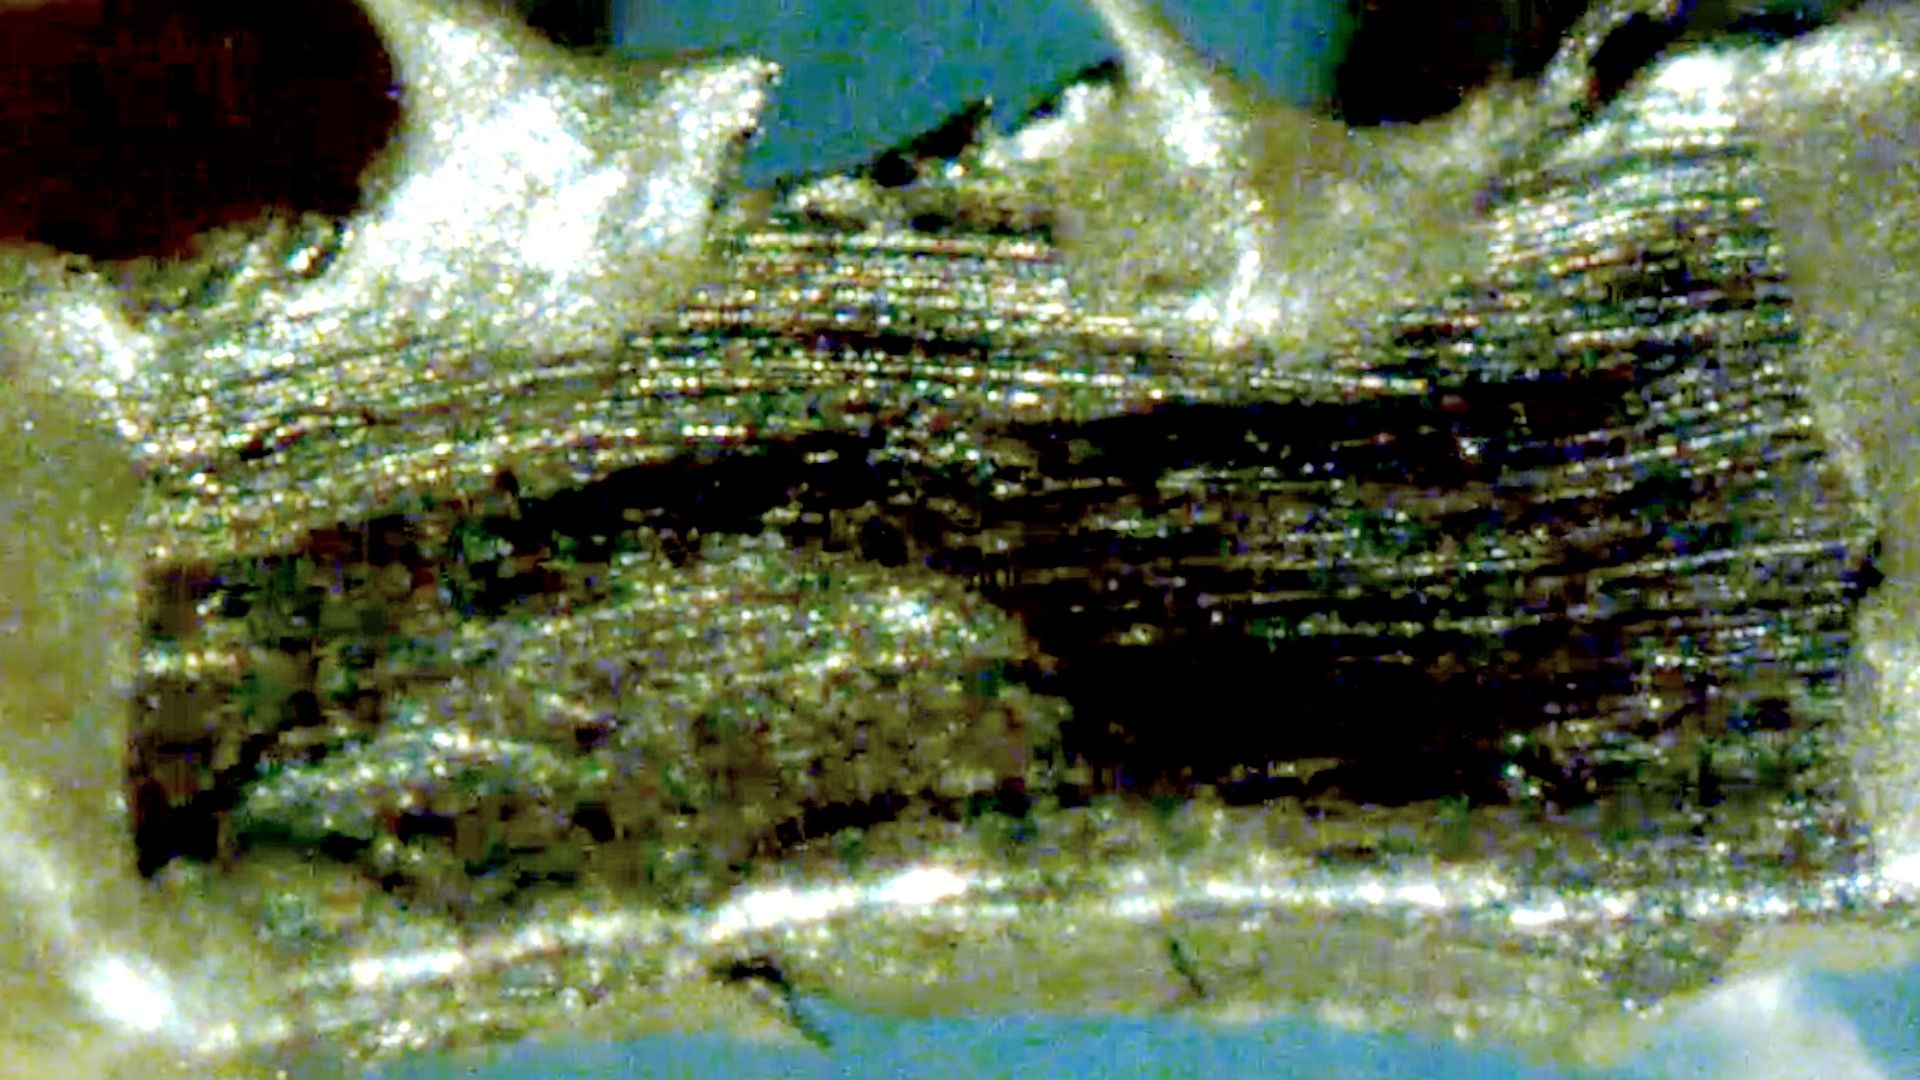
\includegraphics[width=\hsize]{results_discussions/190112_after_pulse17.eps}
  \end{center}
  \caption{}
  \label{fig:190112_after_pulse17}
 \end{minipage}
  \begin{minipage}{0.5\hsize}
  \begin{center}
   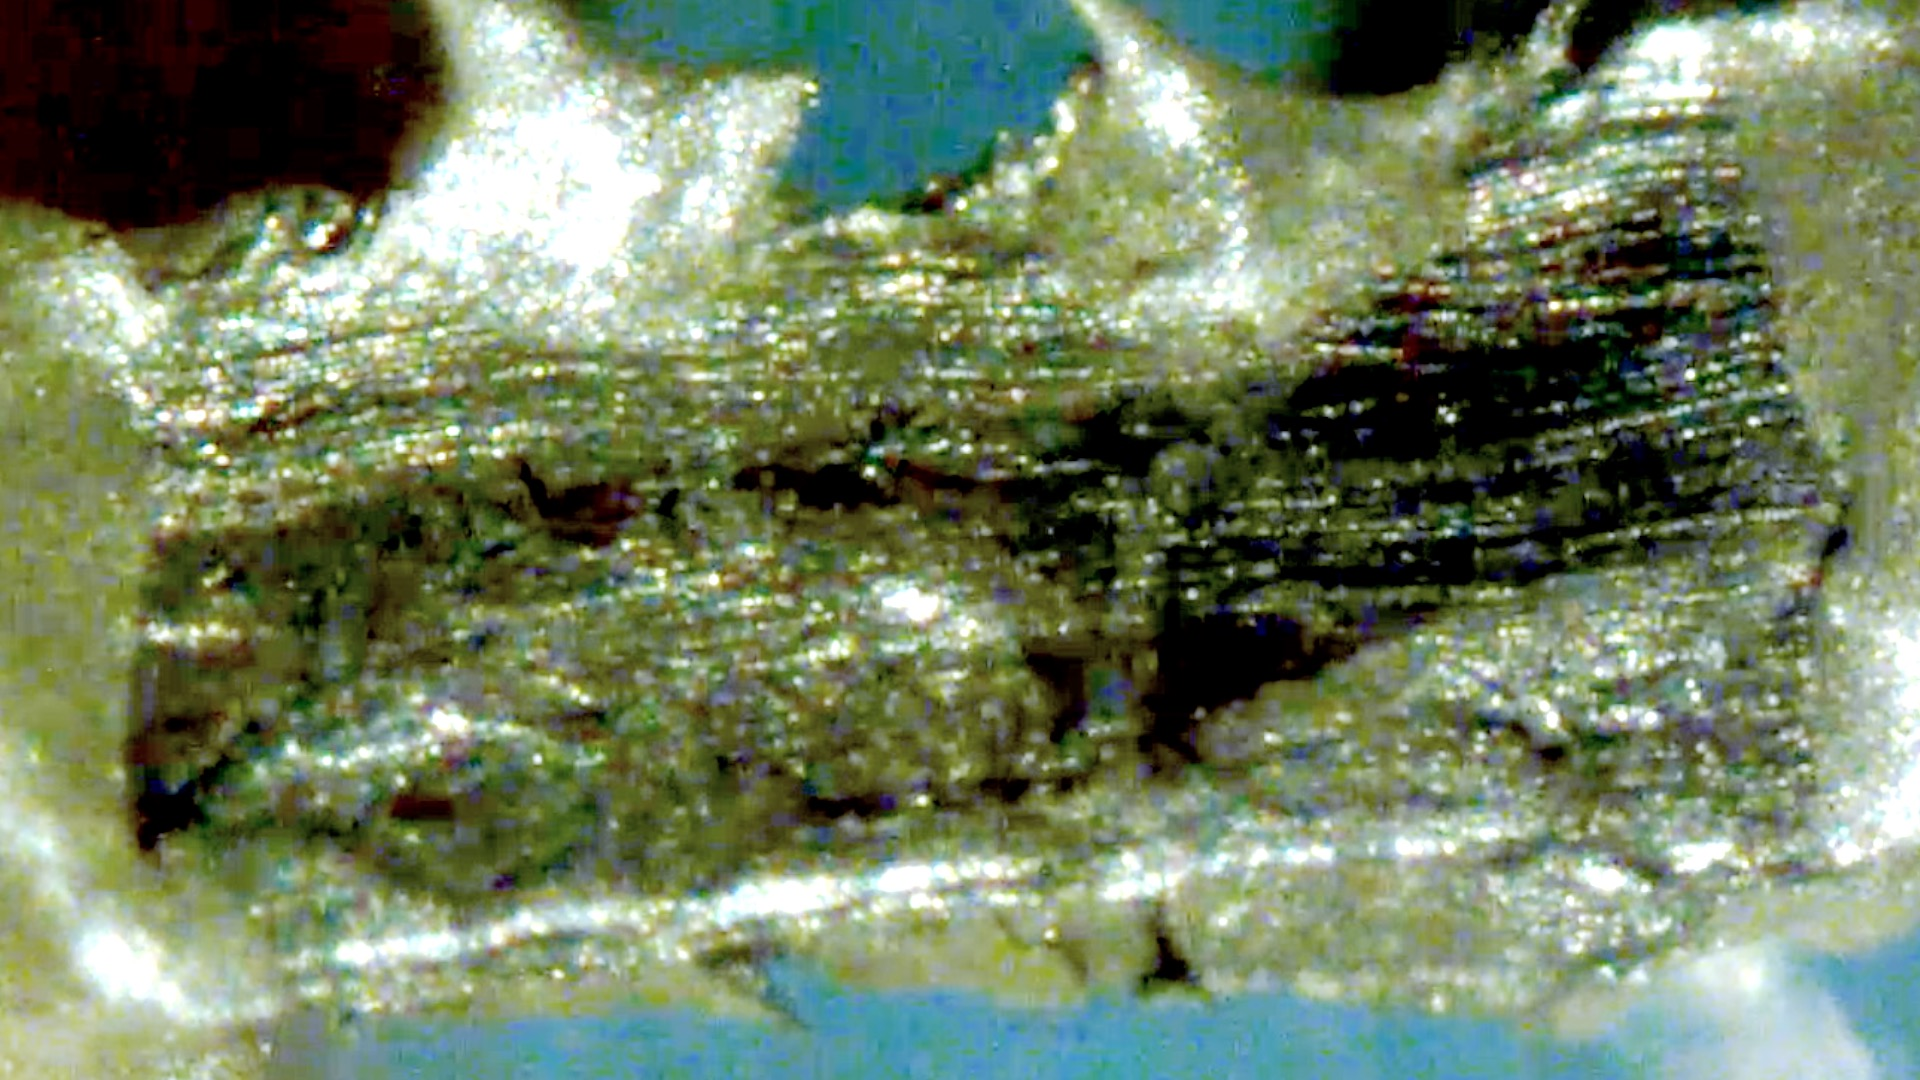
\includegraphics[width=\hsize]{results_discussions/190112_after_pulse19_1.eps}
  \end{center}
  \caption{}
  \label{fig:190112_after_pulse19_1}
 \end{minipage}
  \begin{minipage}{0.5\hsize}
  \begin{center}
   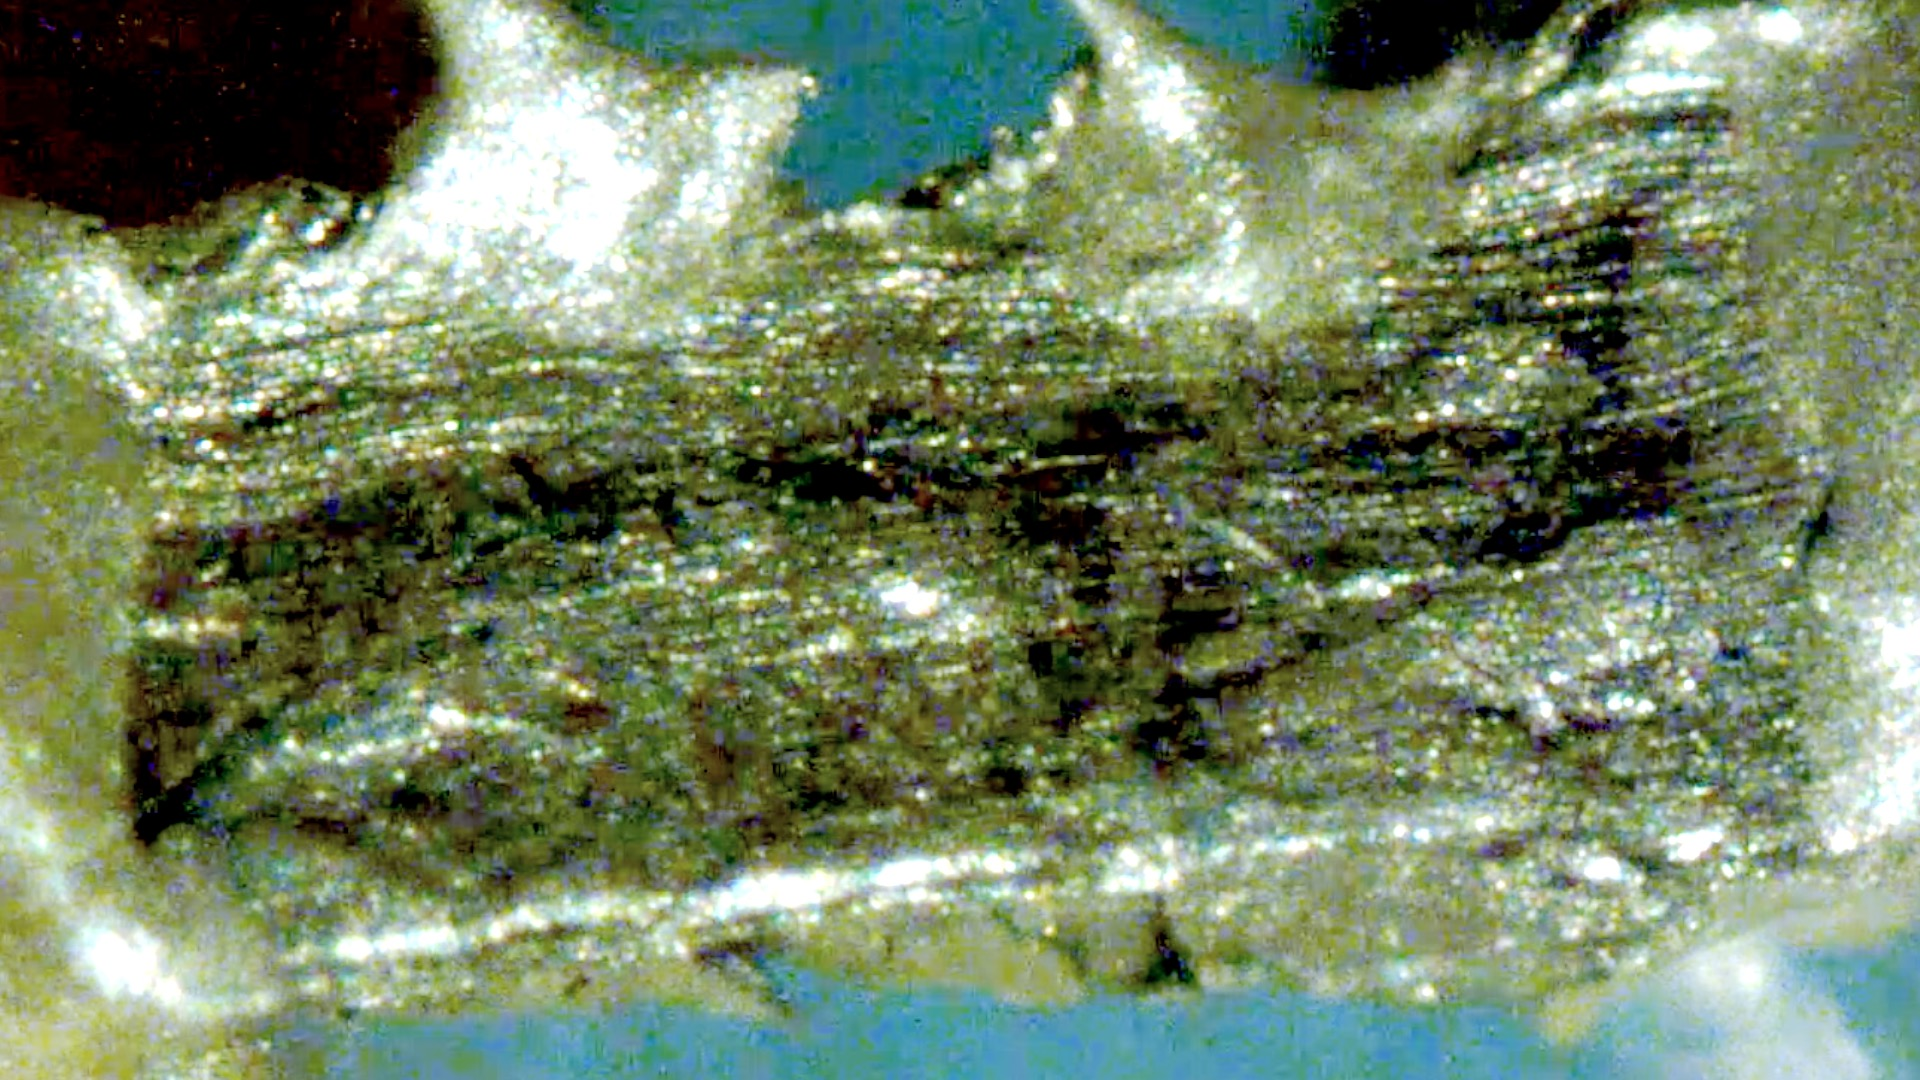
\includegraphics[width=\hsize]{results_discussions/190112_after_pulse19_2.eps}
  \end{center}
  \caption{}
  \label{fig:190112_after_pulse19_2}
 \end{minipage}
  \begin{minipage}{0.5\hsize}
  \begin{center}
   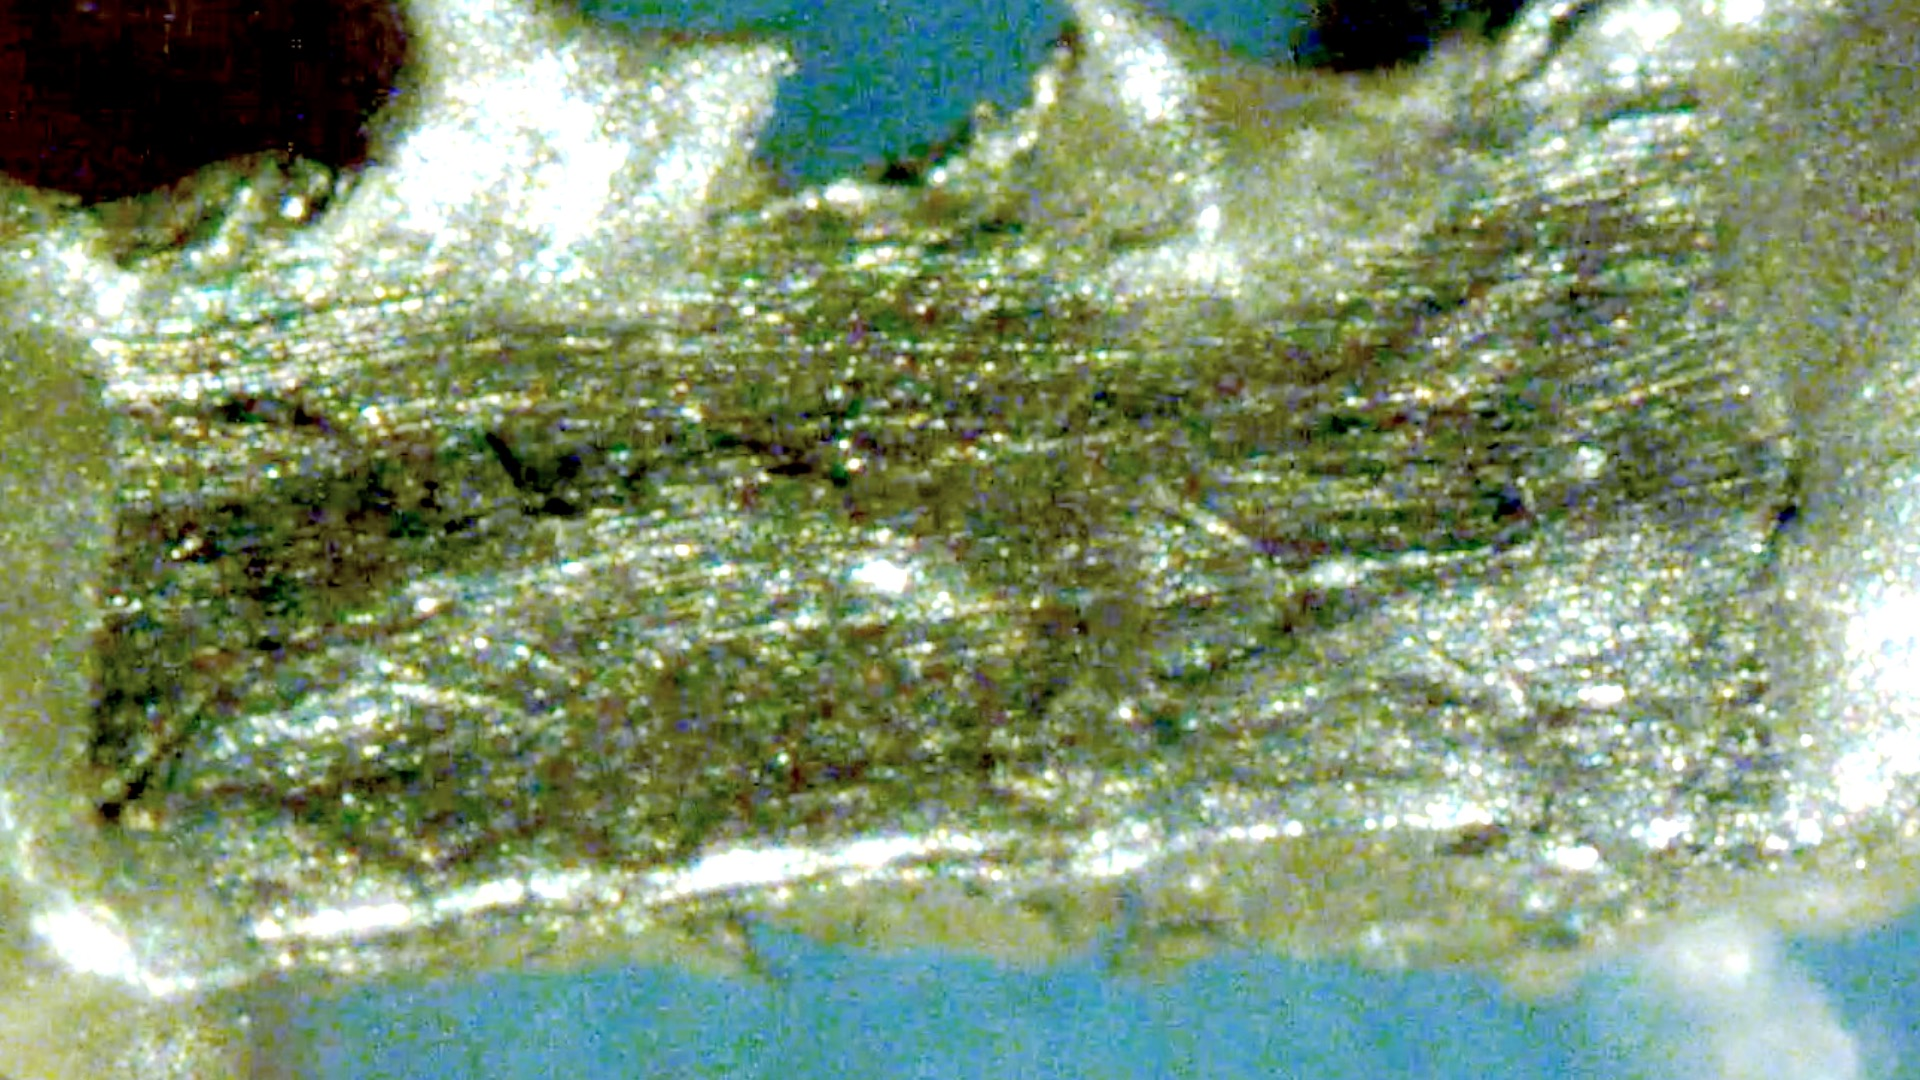
\includegraphics[width=\hsize]{results_discussions/190112_after_pulse20.eps}
  \end{center}
  \caption{}
  \label{fig:190112_after_pulse20}
 \end{minipage}
\end{figure}
No.17のパルス列を印加する前の画像(図\ref{fig:190112_before_pulse17})と全てのパルスを印加した後の画像(図\ref{fig:190112_after_pulse20})を比較すると、黒色の半導体的な吸収を示すαスズから金属的な光沢を持つβスズへの転移がはっきりと見て取れる。また詳しく見ると、相転移は熱の流入源である左側の電流端子から始まり、熱の流出先である二つの電圧端子と右側の電流端子に向かって進行していることがわかる。


\begin{figure}[!h]
 \begin{minipage}{\hsize}
    \begin{center}
   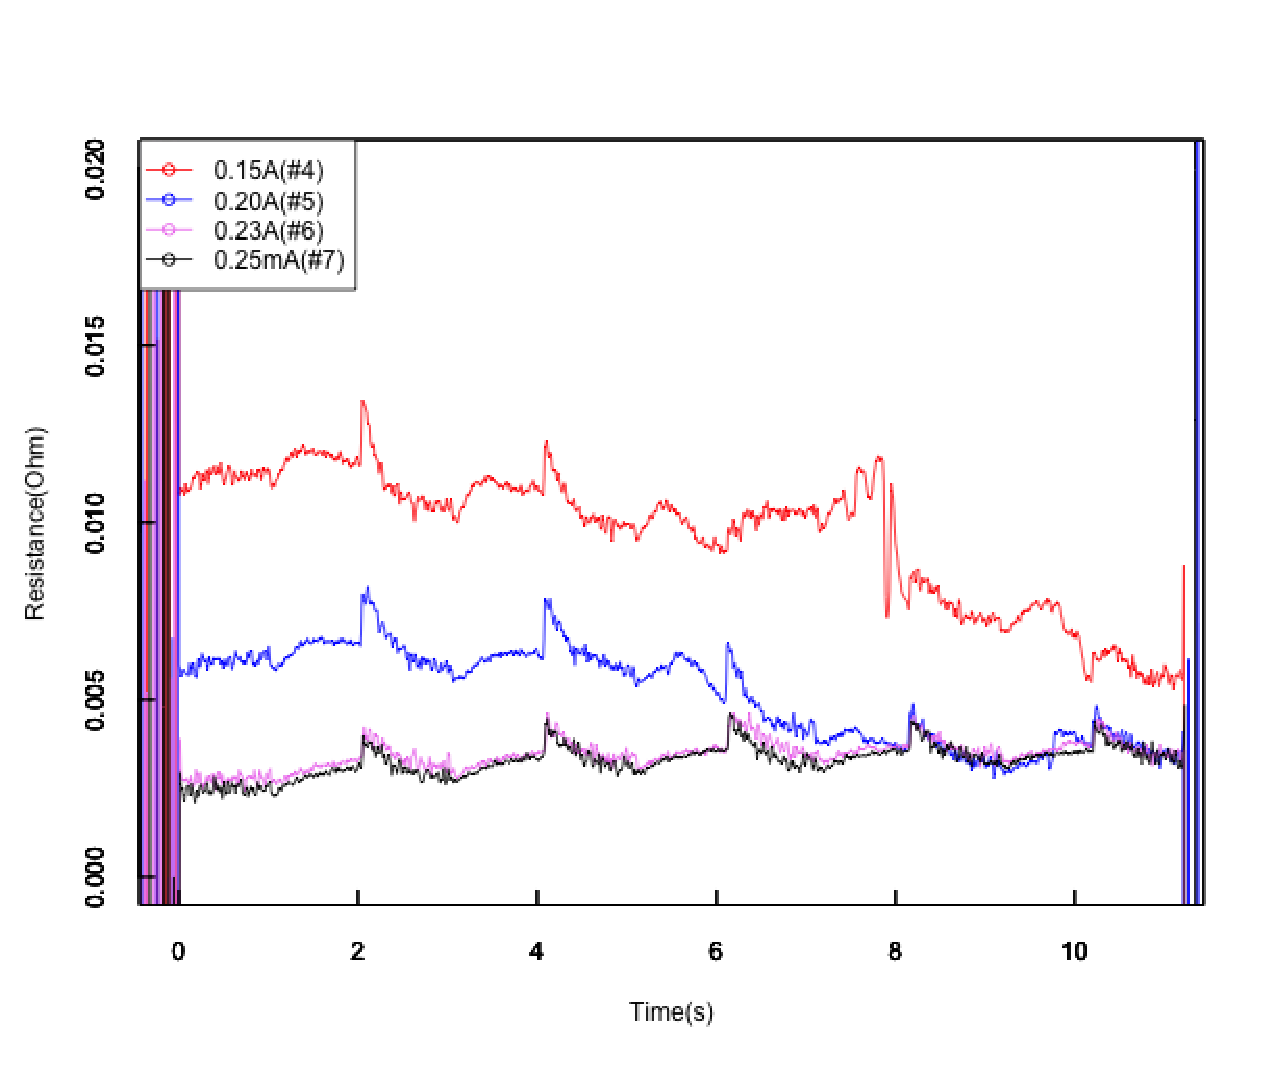
\includegraphics[width=0.9\hsize]{results_discussions/190113_Resistance_pulse.eps}
  \end{center}
  \caption{}
  \label{fig:190113_Resistance_pulse}
 \end{minipage}
 \begin{minipage}{\hsize}
     \begin{center}
   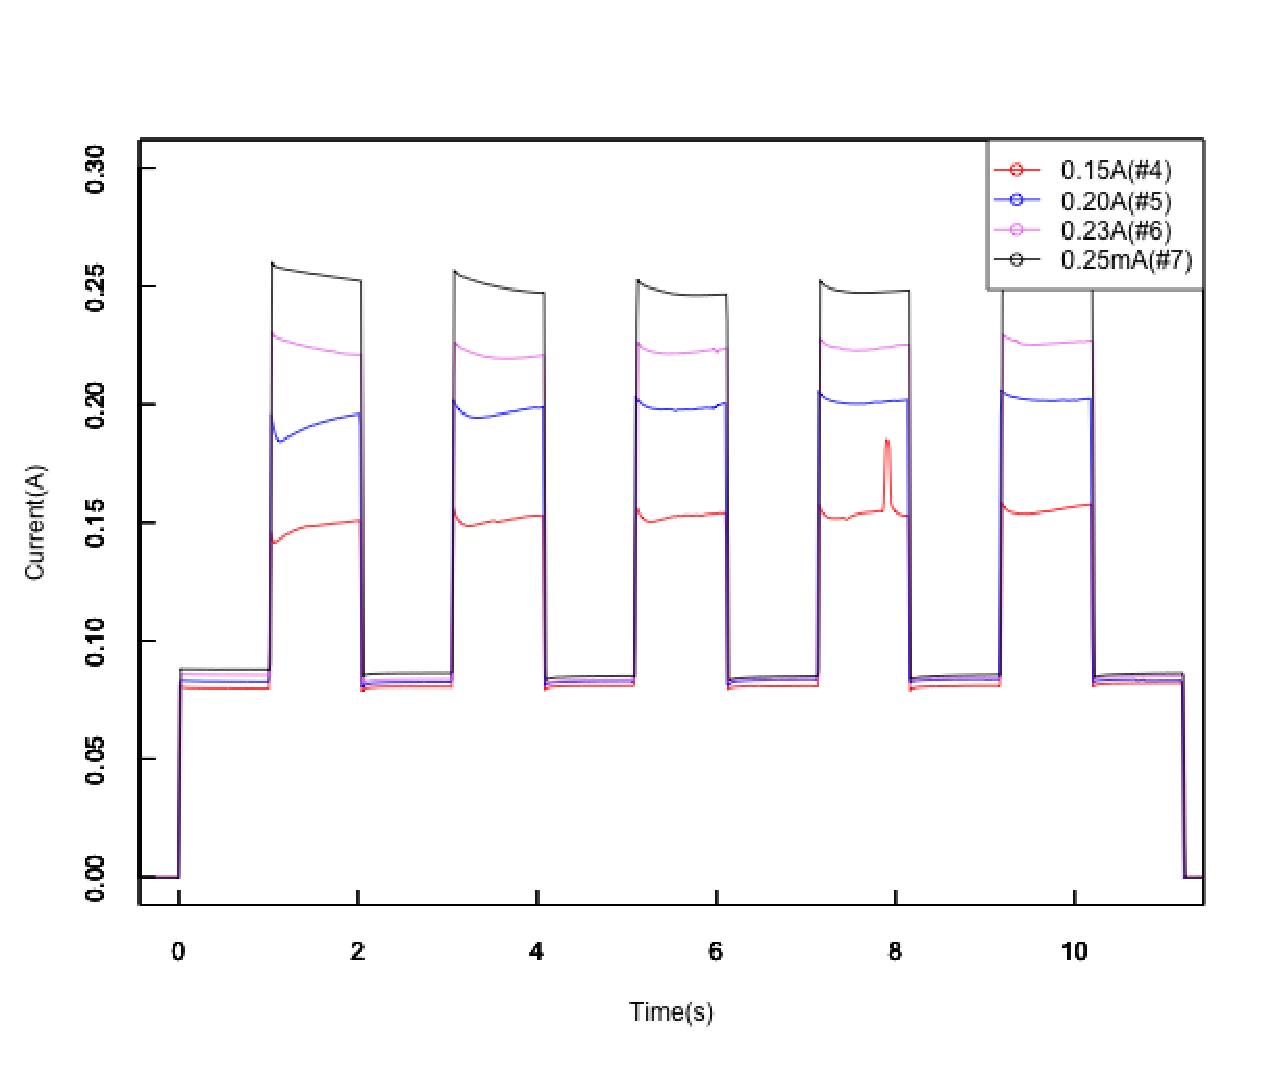
\includegraphics[width=0.9\hsize]{results_discussions/190113_Current_pulse.eps}
  \end{center}
  \caption{}
  \label{fig:190113_Current_pulse}
   \end{minipage}
\end{figure}

\begin{figure}[htbp]
 \begin{minipage}{0.5\hsize}
  \begin{center}
   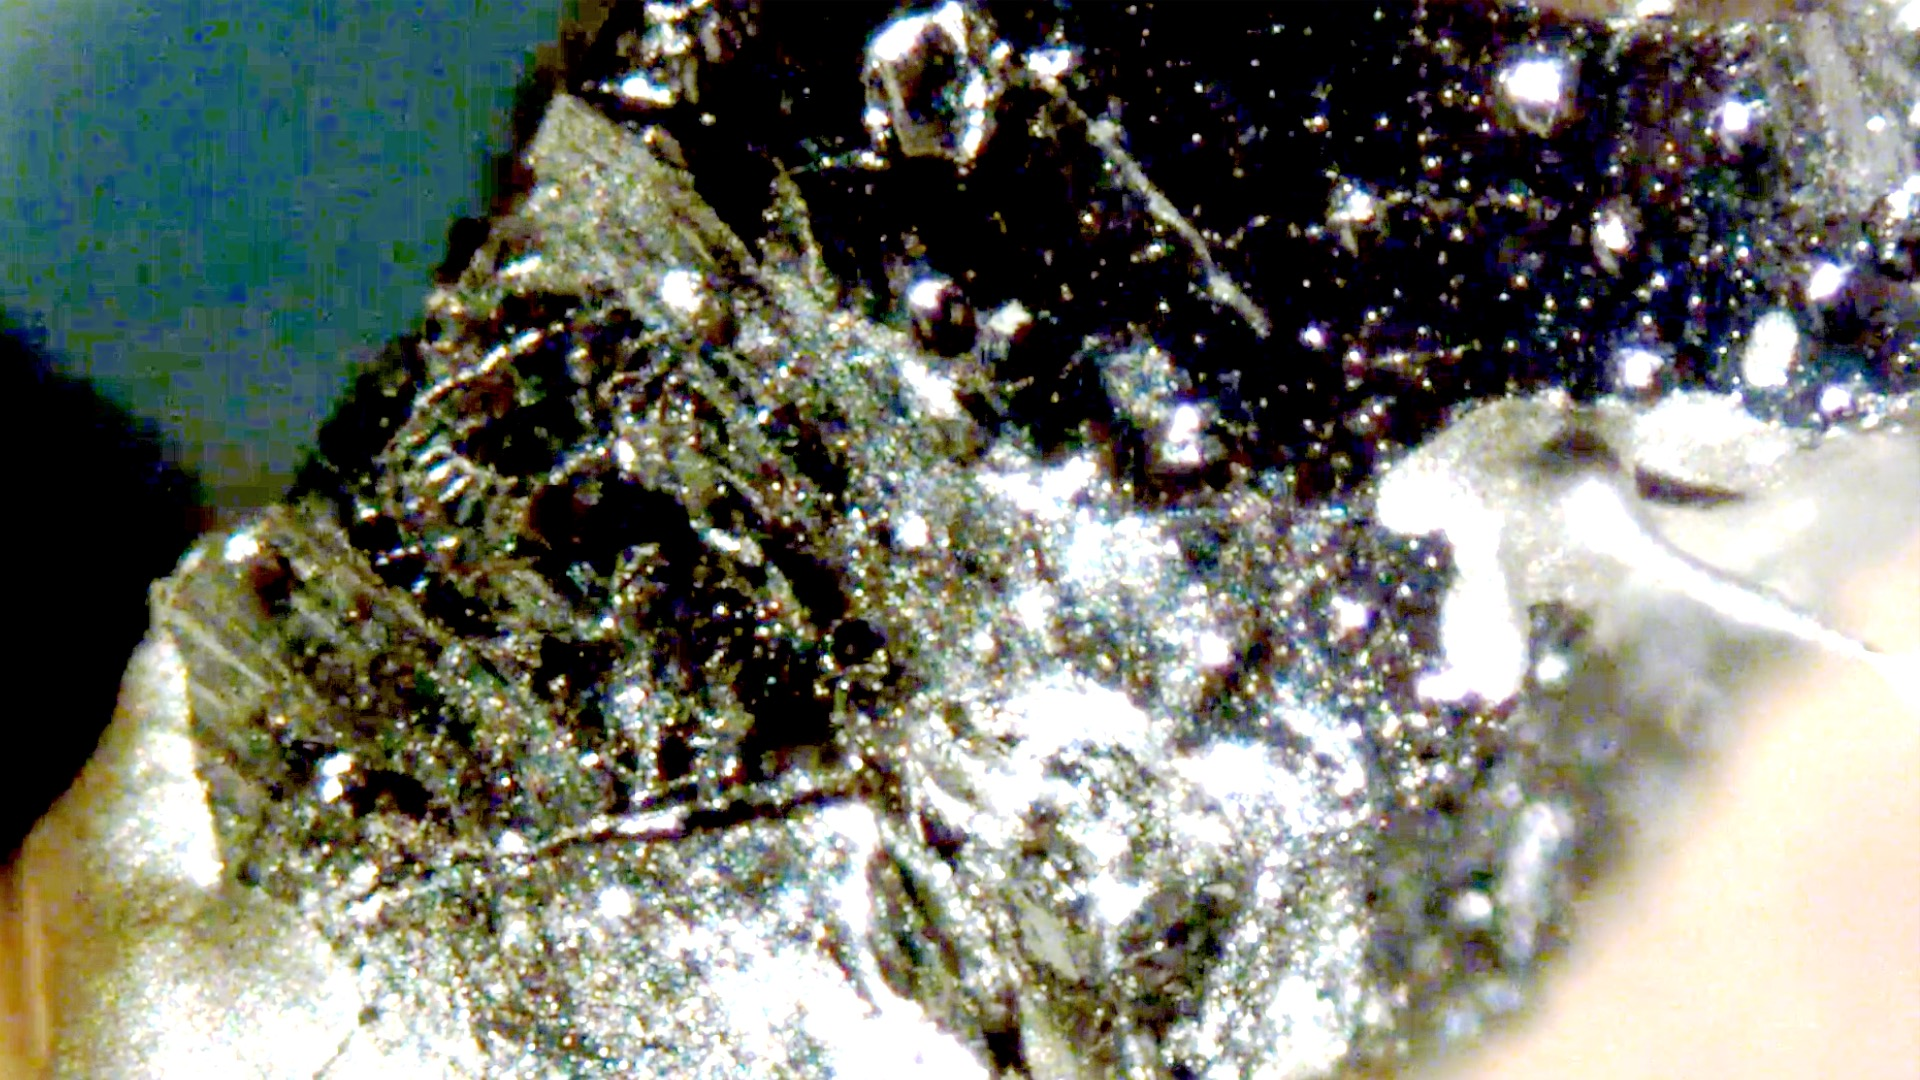
\includegraphics[width=\hsize]{results_discussions/190113_before_pulse5.eps}
  \end{center}
  \caption{}
  \label{fig:190113_before_pulse5}
 \end{minipage}
 \begin{minipage}{0.5\hsize}
  \begin{center}
   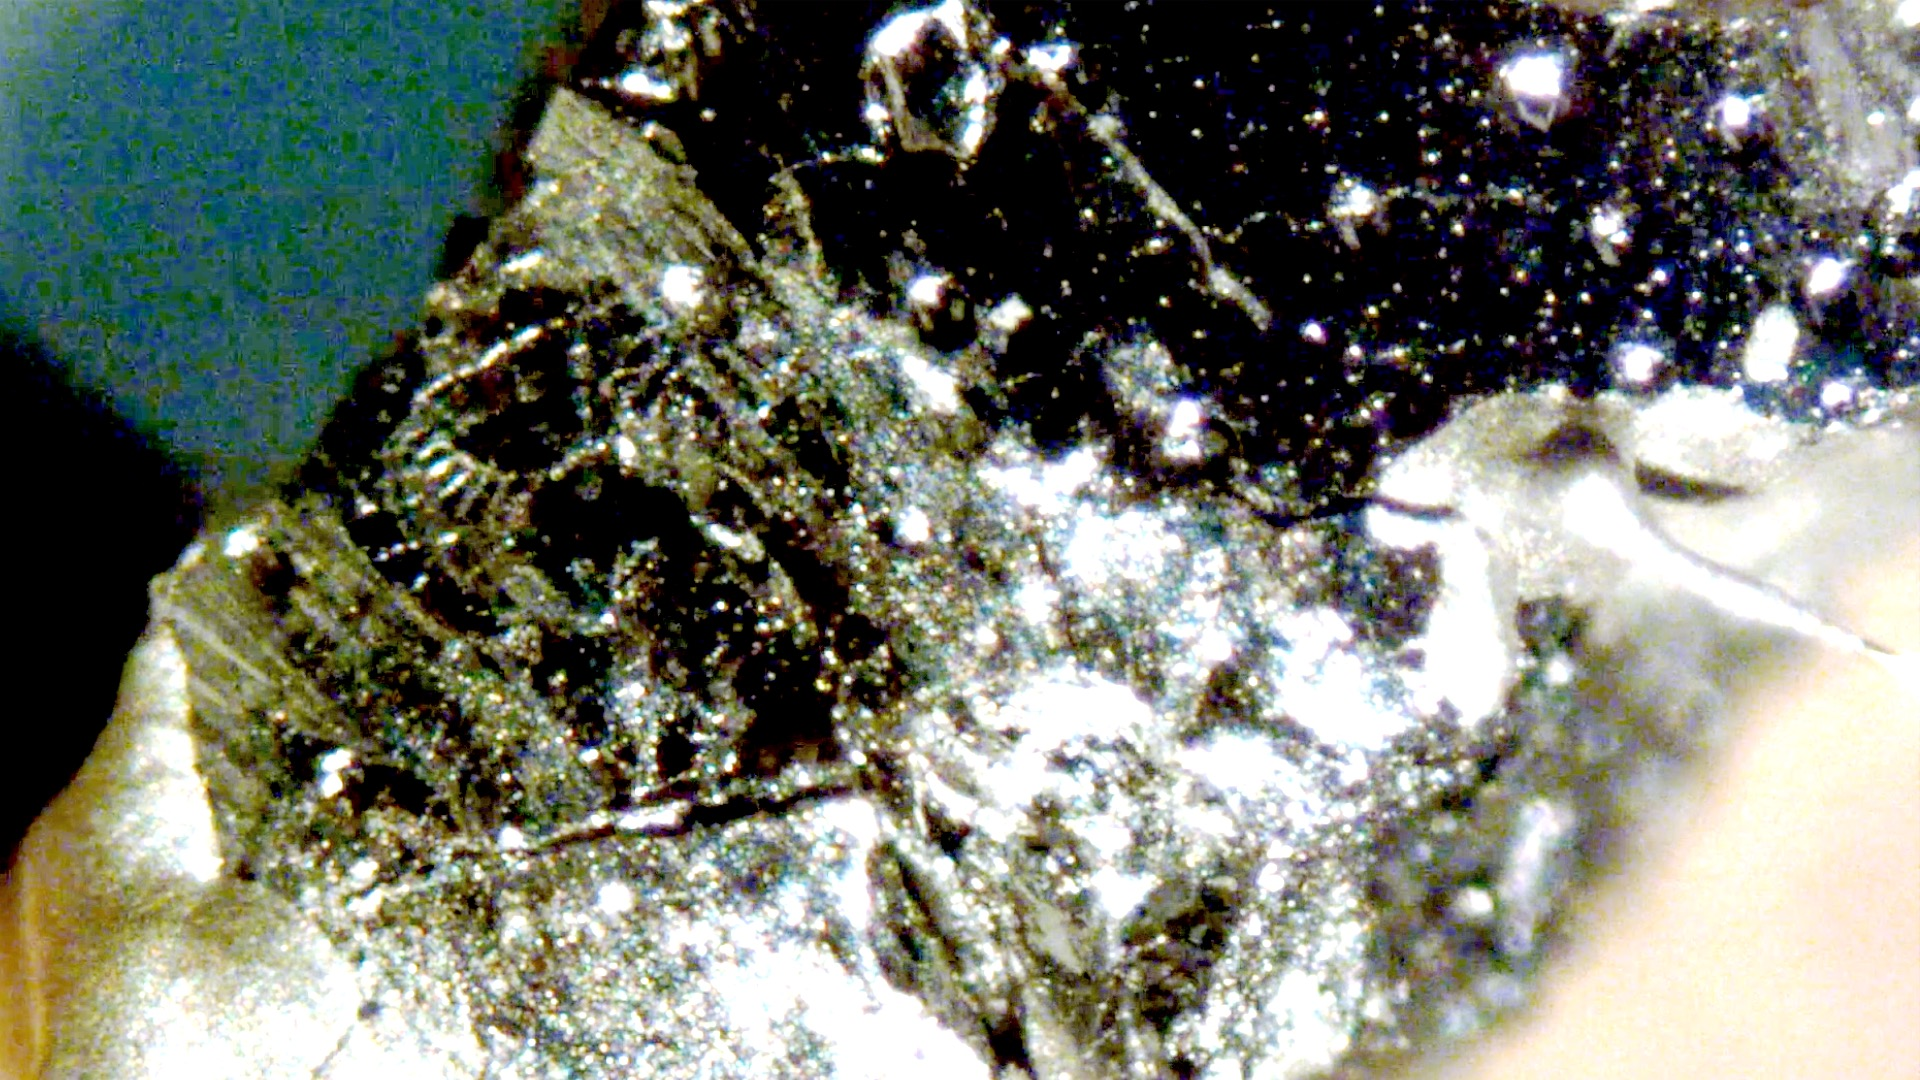
\includegraphics[width=\hsize]{results_discussions/190113_after_pulse5-1.eps}
  \end{center}
  \caption{}
  \label{fig:190113_after_pulse5-1}
 \end{minipage}
  \begin{minipage}{0.5\hsize}
  \begin{center}
   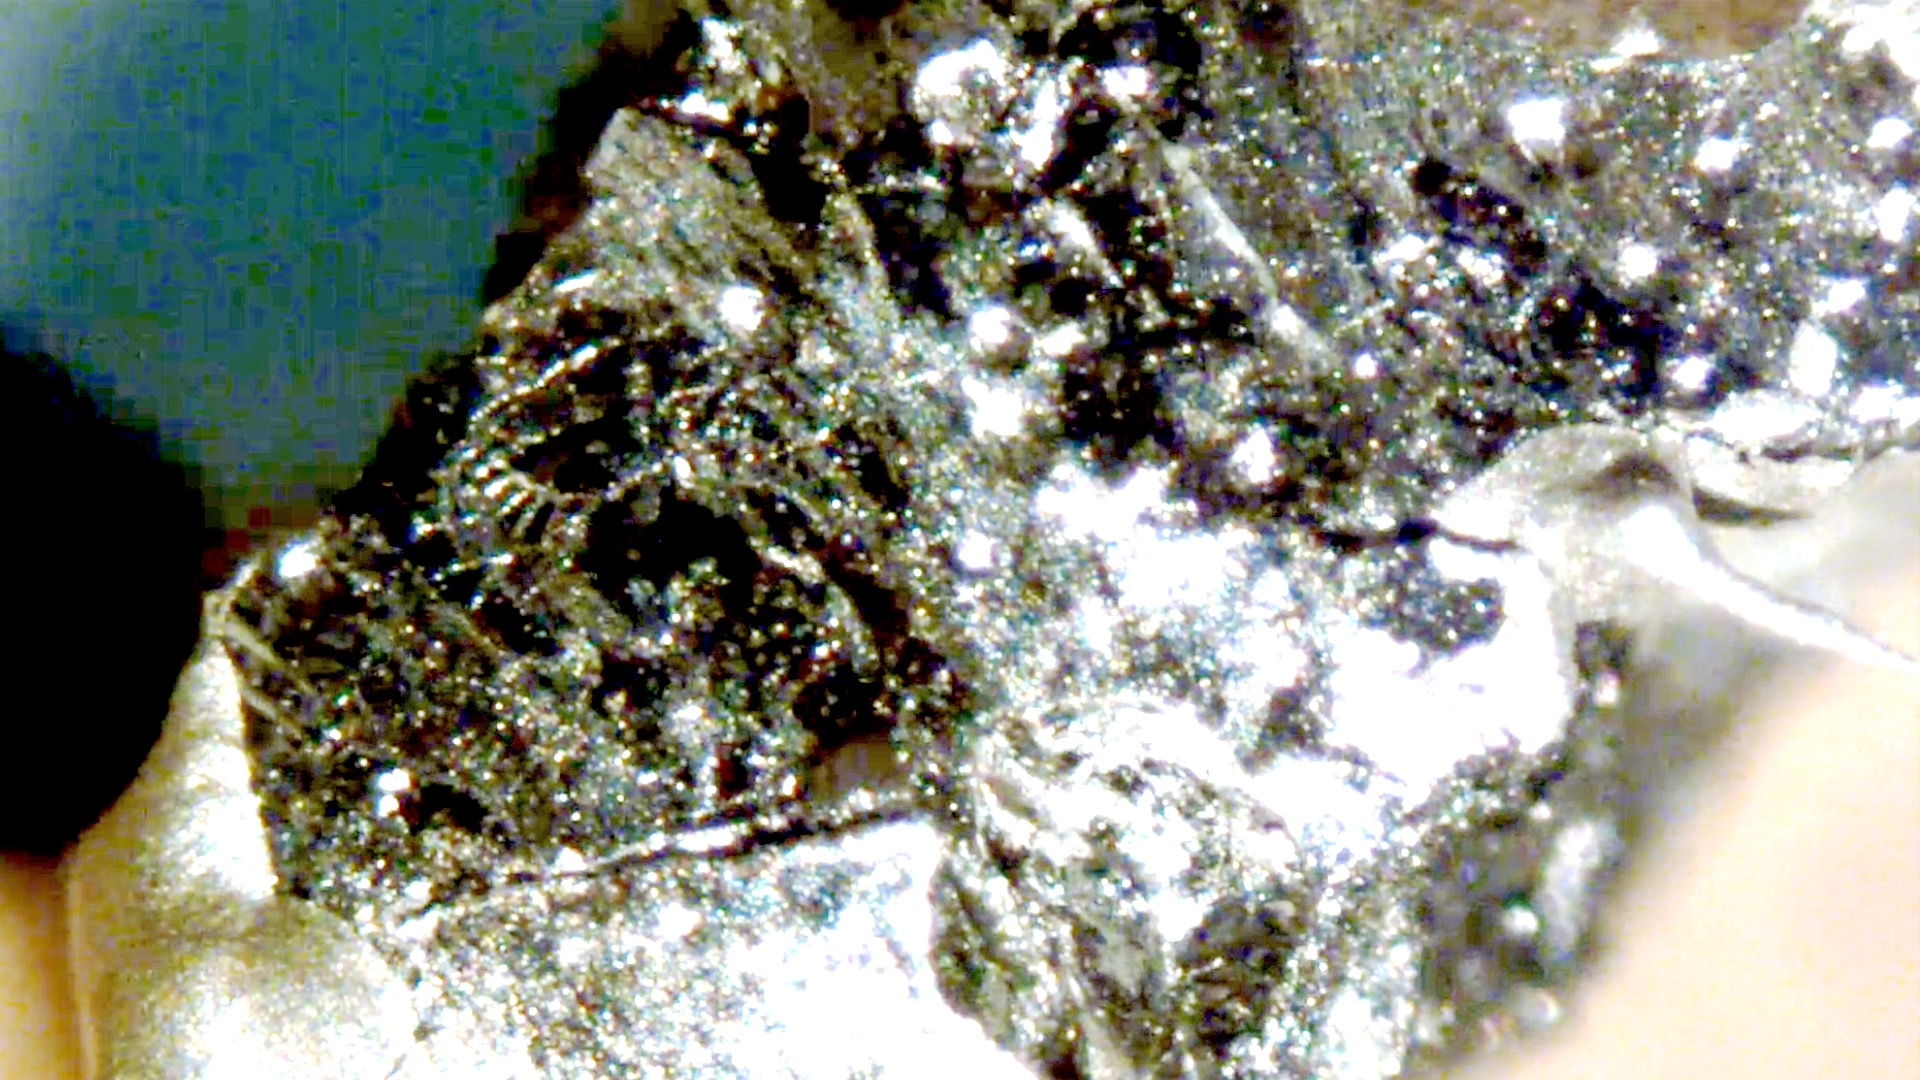
\includegraphics[width=\hsize]{results_discussions/190113_after_pulse5-2.eps}
  \end{center}
  \caption{}
  \label{fig:190113_after_pulse5-2}
 \end{minipage}
  \begin{minipage}{0.5\hsize}
  \begin{center}
   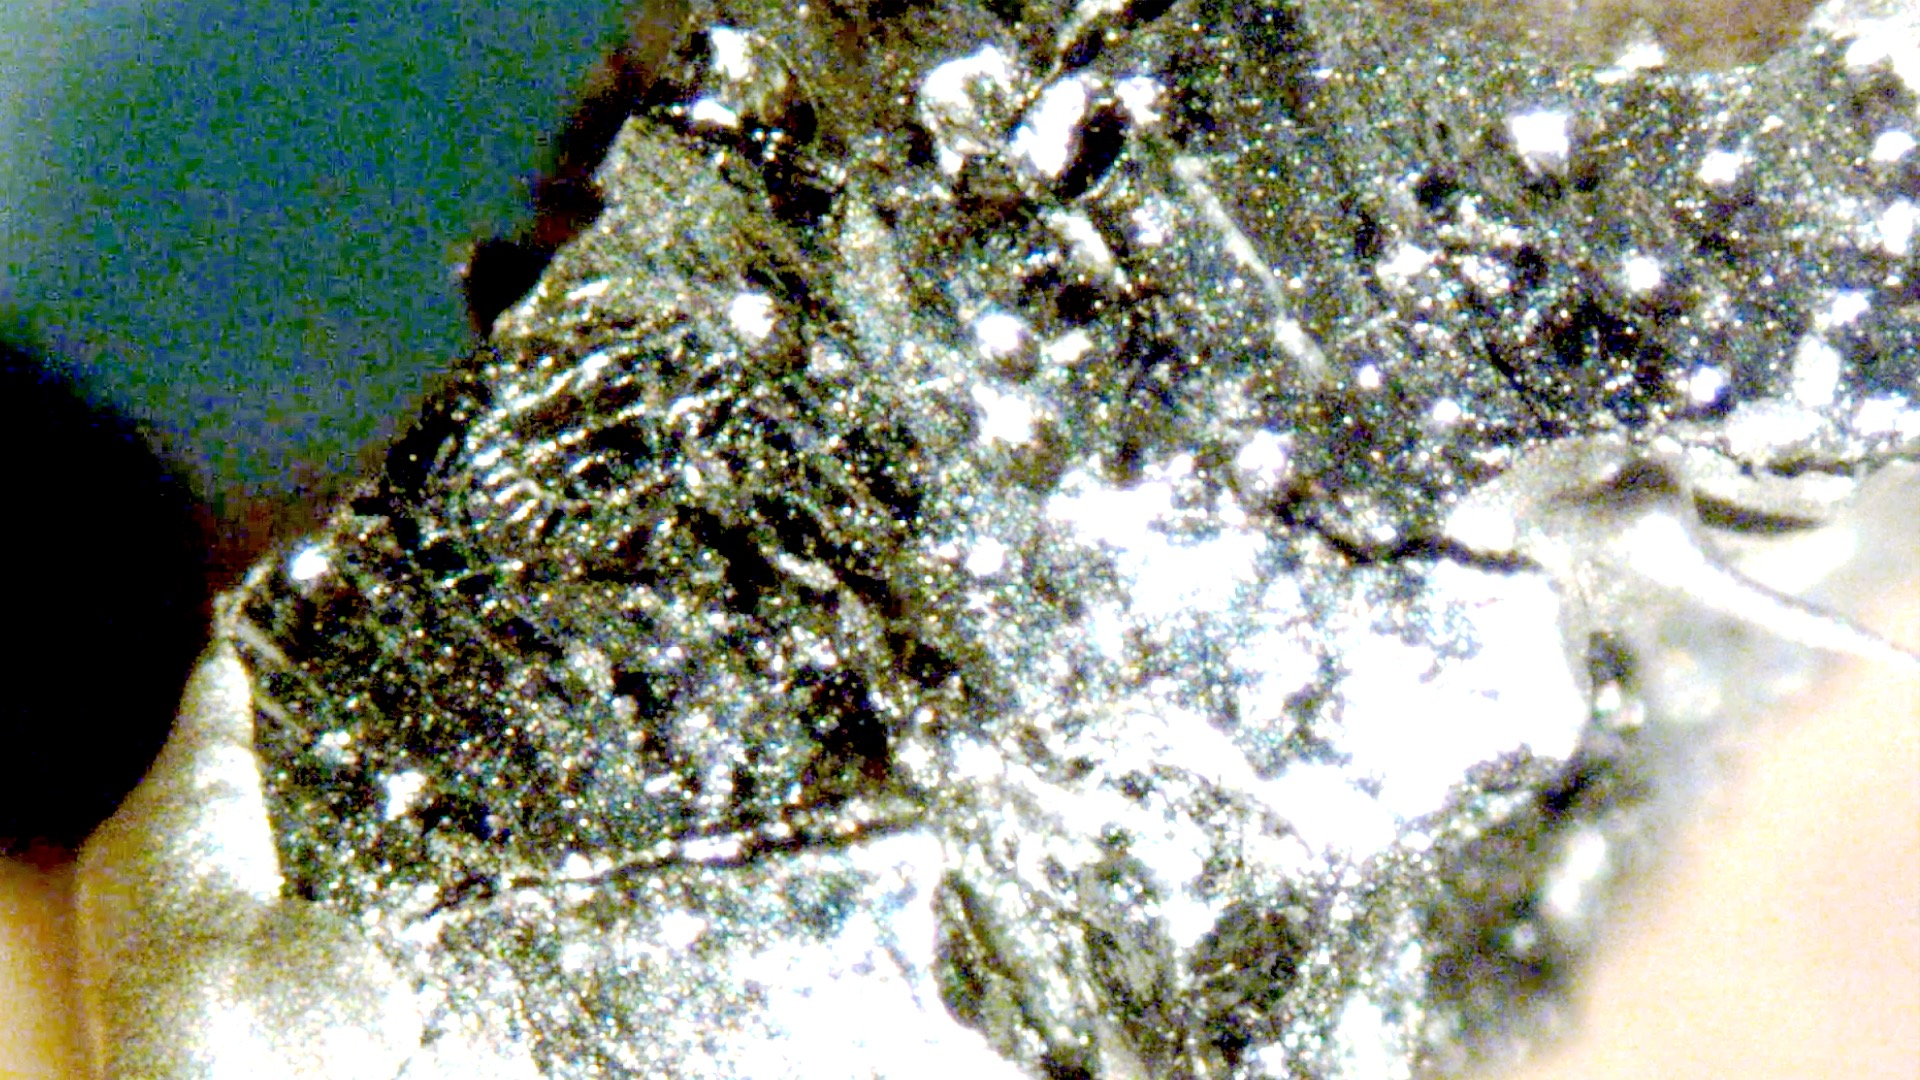
\includegraphics[width=\hsize]{results_discussions/190113_after_pulse5-3.eps}
  \end{center}
  \caption{}
  \label{fig:190113_after_pulse5-3}
 \end{minipage}
  \begin{minipage}{0.5\hsize}
  \begin{center}
   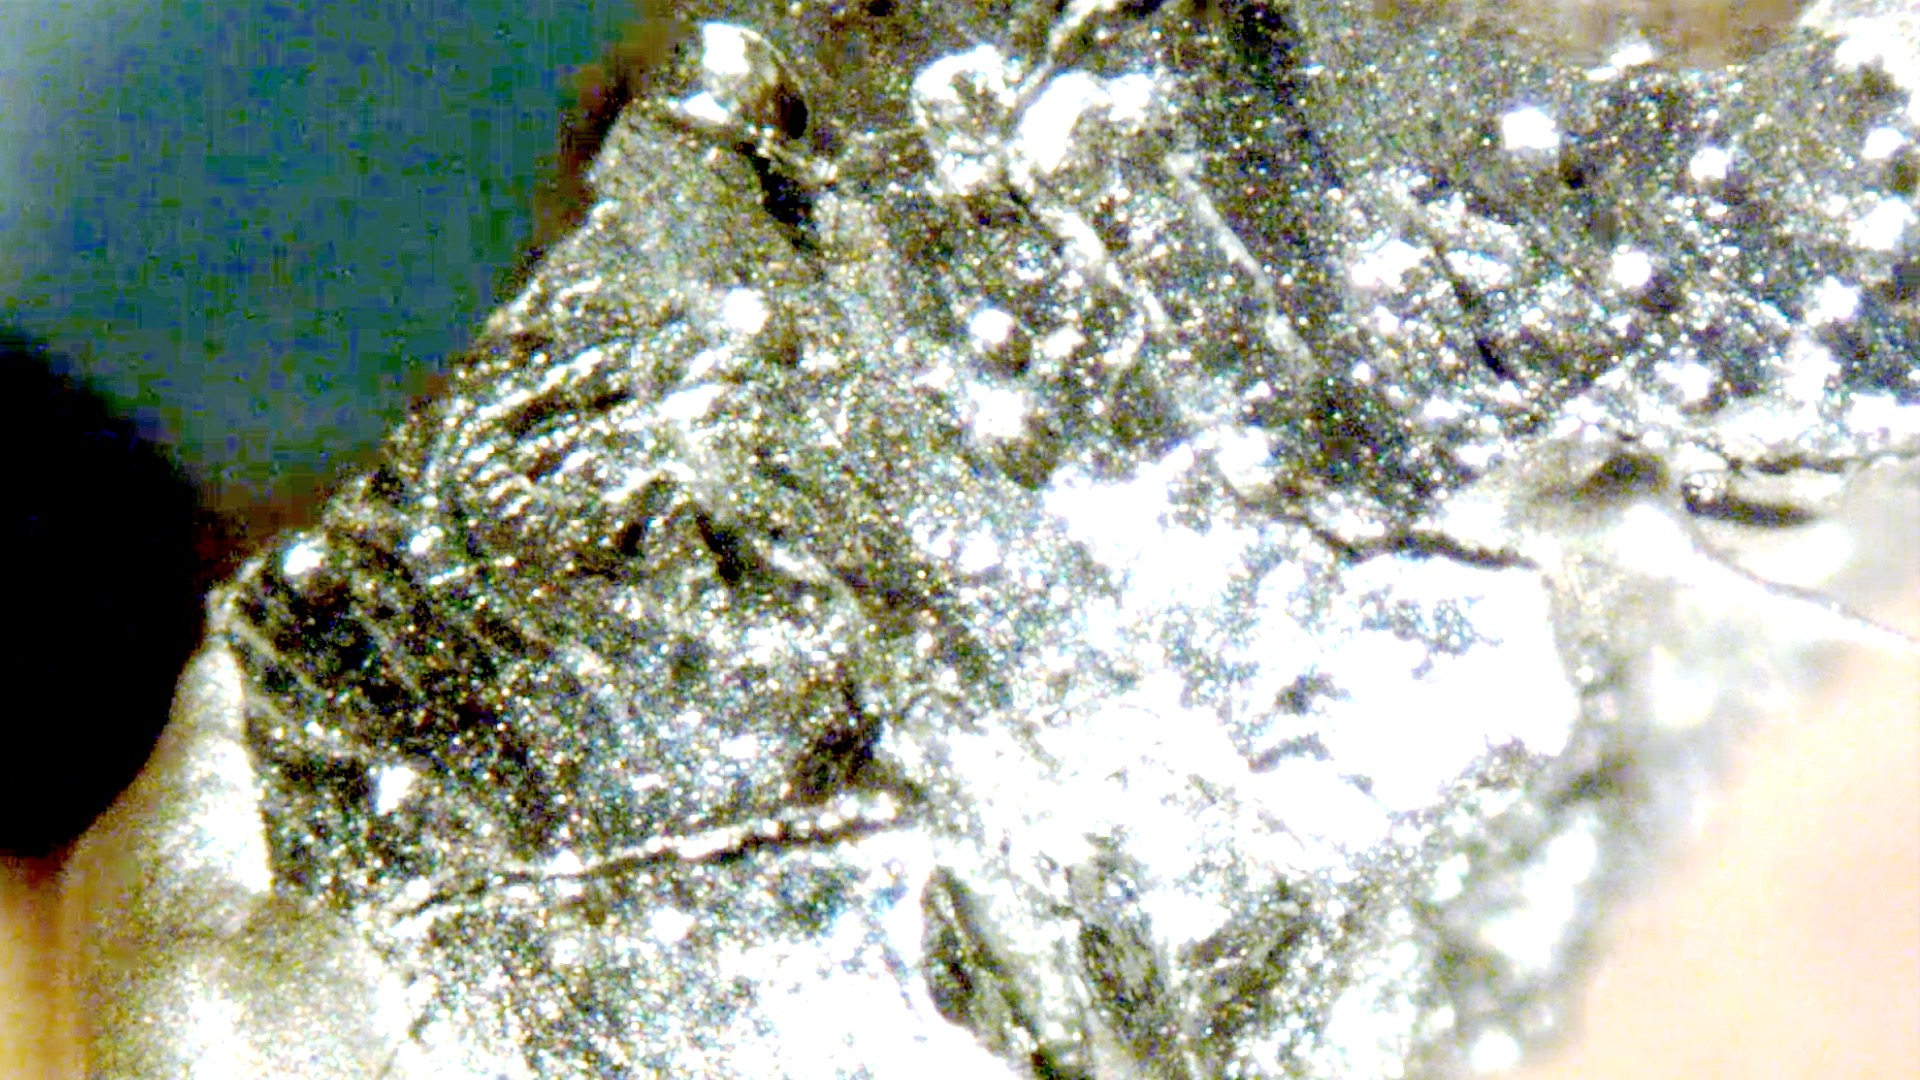
\includegraphics[width=\hsize]{results_discussions/190113_after_pulse6.eps}
  \end{center}
  \caption{}
  \label{fig:190113_after_pulse6}
 \end{minipage}
\end{figure}


%\subsection{電流パルスを用いたβ相からα相への変換}

\clearpage

%cd Documents/GitManagedProjects-Kagawalab/報告書/卒業論文/results_discussions/